\section{Classifier Evaluation}
\subsection{Confusion Matrix}
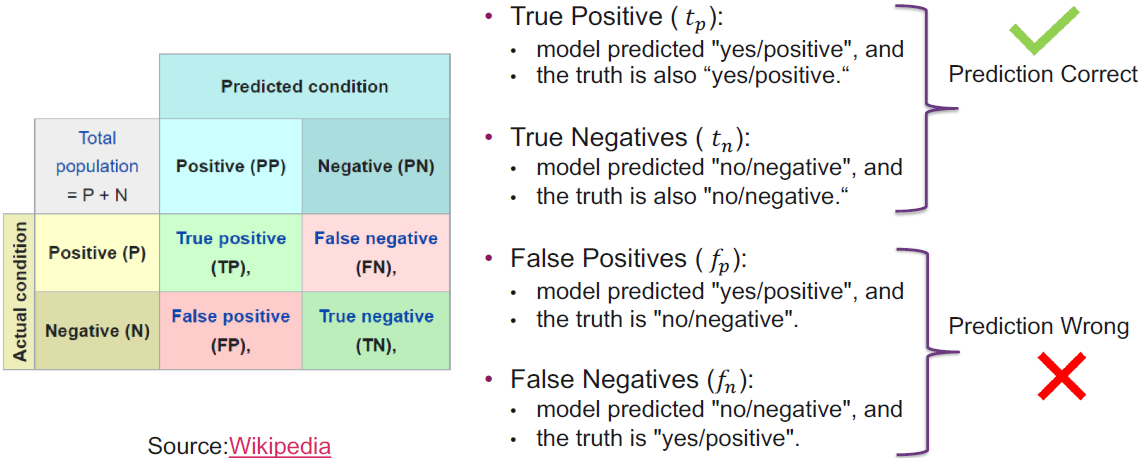
\includegraphics[width=\linewidth]{confusion_matrix.png}
\textbf{Mean Accuracy}
\begin{itemize}
    \item How often is the classifier correct?
    \item $A = (t_p + t_n) / n$
\end{itemize}
\textbf{Mean Error}
\begin{itemize}
    \item How often is the classifier wrong?
    \item $E = (f_p + f_n) / n$
\end{itemize}
\textbf{Precision}
\begin{itemize}
    \item When the prediction is 1, how often is it correct?
    \item $P = t_p / (t_p + f_p)$
\end{itemize}
\textbf{Sensitivity, Recall, True Positive Rate (TPR)}
\begin{itemize}
    \item How often the prediction is 1 when it's actually 1
    \item $R = t_p / (t_p + f_n)$
\end{itemize}
\textbf{Miss Rate, False Negative Rate (FNR)}
\begin{itemize}
    \item $MR = 1 - TPR$
\end{itemize}

\subsection{Why Accuracy is not enough?}
\begin{itemize}
    \item If the prediction is constant the accuracy may still look decent
    \item E.g. always predict false
    \item 90\% of the data is false
    \item Accuracy = 90\% (decent)
    \item Precision = 0
    \item Recall = 0
\end{itemize}

\subsection{Precision vs. Recall}
\begin{itemize}
    \item Increasing precision reduces Recall and vice versa
    \item Threshold is a business decision (depending on goals)
\end{itemize}

\subsection{Receiver Operating Characteristics (ROC)}
\begin{itemize}
    \item Defined by FPR and TPR as x and y axes
    \item Visualizes tradeoff between TP (benefits) and FP (cost)
\end{itemize}
\begin{center}
    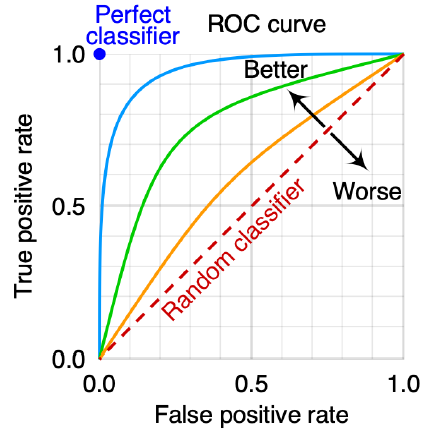
\includegraphics[width=0.4\linewidth]{roc.png}
\end{center}
\textbf{Area under the curve}
\begin{itemize}
    \item Area under the ROC curve
    \item Shows how well the TPR and FPR is looking in the aggregate
    \item The greater the area under the curve, the higher the quality of the model
    \item The greater the area, the higher the ratio of TP to FP
\end{itemize}
